% Enable warnings about problematic code
\RequirePackage[l2tabu, orthodox]{nag}

\PassOptionsToPackage{utf8}{inputenc}
\PassOptionsToPackage{T1}{fontenc}
\PassOptionsToPackage{ngerman, american}{babel}

\hyphenation{Prefix-queries}
\title{Fast and Non-Approximative \mbox{Language Model Prefixqueries} for Word Prediction using Top-k Joining Techniques}
%\title{Exemplary solving Noisy Channel Type Queries: Next Word Prediction with Keystroke savings using Language Models and Top-\textit{k} Joining Techniques}
%\title{Exemplary solving Noisy Channel Type Queries:Next Word Prediction using Top-\textit{k} Joining Techniques}
%\title{Computing Language Model Arg-Max-Queries Using Top-\emph{k} Joining Techniques <WORKING TITLE>}
\author{Lukas Schmelzeisen}
\date{\today}

\documentclass[m,bachelor,classicthesis,classicthesistitle]{thesis}

\authormail{lukas@uni-koblenz.de}
\degreecourse{Informatik}
\firstreviewer{Prof.~Dr.~Steffen Staab}
\firstreviewerinfo{Institute for Web Science and Technologies}
\secondreviewer{Ren{\'e} Pickhardt}
\secondreviewerinfo{Institute for Web Science and Technologies}

\usepackage{pdflscape}
\usepackage{standalone}
\usepackage{tikz}
\usepackage{pgfplots}
\pgfplotsset{compat = 1.12}

% TODO
\usepackage{nicefrac}
\usepackage{paralist}
\newcommand{\inlinecode}[1]{\lstinline[columns=fixed]{#1}}

\addbibresource{bibliography.bib}

% Editorial Commands ===========================================================
% TODO: remove before relase

\usepackage[
  linecolor = Maroon,
  bordercolor = Maroon,
  backgroundcolor = White
]{todonotes}

\definecolor{draft}{rgb}{0.5, 0.5, 0.5}
\newenvironment*{draft}{%
  \color{draft}%
}{%
}

\newcommand*\Lukas[2][]{
  \todo[linecolor = Cyan, bordercolor = Cyan, #1]{\textcolor{Cyan}{Lukas}: #2}
}
\newcommand*\Rene[2][]{
  \todo[linecolor = Blue, bordercolor = Blue, #1]{\textcolor{Blue}{Rene}: #2}
}

\newcommand{\noref}{\textcolor{RoyalBlue}{\footnotesize[Citation needed]}}
\newcommand{\mbref}[1]{\textcolor{RoyalBlue}{\footnotesize[Citation: #1?]}}

% ==============================================================================

\begin{document}
\frenchspacing
\raggedbottom

% Frontmatter ==================================================================

\pagestyle{scrplain}
\pagenumbering{roman}

\selectlanguage{ngerman}
\maketitle
\selectlanguage{american}

\cleardoublepage
\pdfbookmark[1]{Abstract}{Abstract}
\begin{abstractpage}
  \begin{abstract}
    \todo[inline]{Write Abstract.}

    Next word prediction is the task of guessing the next word a user intends to
    type from the words they have already entered.
    Traditionally this problem is solved by calculating an argmax of language
    model probabilities for all words in a vocabulary.
    However this approach is slow and becomes linearly worse with
    increasing vocabulary size.
    This thesis proposes two independent optimizations.
    First, a novel approach is presented that allows to move a part of
    probability calculation into a precomputation step.
    Second it is shown how to apply top-k joining techniques to word
    prediction to avoid enumerating all words in the vocabulary.
    Using both optimizations sub-millisecond next word prediction time is
    achieved.

    \begin{draft}
      The concern of this thesis is solving noisy channel type queries that are based
      on statistical language model probabilities.
      Our novel approach is to formulate language models as weighted sum functions on
      occurrence counts.
      As these weighted sum functions are monotone, we can then employ various
      top-$k$ joining techniques, to efficiently find those arguments that maximize
      the noisy channel's probability.
      This approach can be used for all noisy channel type queries, that can be
      expressed as monotone scoring functions.
      We will present our method by implementing next word prediction with it.
    \end{draft}
  \end{abstract}

  \selectlanguage{ngerman}
  \begin{abstract}
    \todo[inline]{{\"U}bersetzte Abtract auf Deutsch.}
  \end{abstract}
  \selectlanguage{american}
\end{abstractpage}



\clearpage
\todo[inline]{License!}
\todo[inline]{Dedication}
\todo[inline,caption={Discussion with Ren{\'e}}]{
  Discussion with Ren{\'e}:
  \begin{itemize}
    \item Terminology: Probability event?
  \end{itemize}
}
\todo[inline]{Use etoolbox for ifthenelse in class.}
\todo[inline]{Kill warnings.}
\todo[inline]{Rewrite math package. Use left/right braces for set.}
\todo[inline]{Use subequations more often?}
\todo[inline, caption={Check for typographicals errors before submission.}]{%
  Check for typographical errors before submission.%
  \begin{itemize}%
    \item Check if all ellipsis "\ldots" are done using
      \texttt{\textbackslash{}ldots}.%
    \item Check if words ending in "s" require possessive apostrophe.%
  \end{itemize}%
}
\todo[inline]{Keywords?}

\section*{Title}

Are my prefixqueries actually correct? It sound like I address the problem
of formulating the correct query, not solving it correctly. Also do I actually
solve correctly? Only TA does, NRA and BS are approximations.

Wanted to avoid comparision, cause it sounds like I have zero own contribution.

Do I include phrase "using top-k joining techniques". My BS won't be based on
top-k joining.

\cleardoublepage
\pdfbookmark[1]{\contentsname}{toc}
\tableofcontents

% Mainmatter ===================================================================

\cleardoublepage
\pagenumbering{arabic}
\pagestyle{scrheadings}

\chapter{Introduction}
\label{ch:introduction}

\todo[inline]{
  Rewrite introduction with new title in mind:
  NWP is important.
  NWP is hard and slow.
  NWP quality is measured with NKSS.
  NWP and NKSS form prefix queries.
  I make fast prefix queries.
}

\begin{draft}
\textcite{Bickel2005} actually does trivial argmax and calculates probabilities
for all words in vocabulary repeatedly.
\end{draft}

The \emph{noisy channel model} is a commonly applied concept in natural language
processing.
As first described by \textcite{Shannon1948}, it consists of a transmitter that
tries to pass a message over a channel to a receiver.
The channel is called noisy, because it may distort the message in any way.
The task is then to reconstruct the original message, from the recieved,
distorted one.

This metaphor has many applications, such as spelling correction
\parencite{JurafskyMartin2009,Manning2008,Kernighan1990,Mays1991},
%          \------------- non-word-errors ------------/    \- real-word-erros
word prediction \parencite{Bickel2005}, part-of-speech tagging
\parencite{Church1988}, machine translation \parencite{Brown1990}, speech
recognition or text compression.
\todo{Newer citations!}
% JurafskyMartin2009: Chapter 5: Spelling Correction
%                     Chapter 9: Speech Recognition!

This thesis will present a novel approach to solve noisy channel type queries.
The basic idea is to formulate the query as the argmax of a monotone scoring
function, and then to find the solution using \emph{top-$k$ joining techniques}.
This approach will exemplary be showcased by applying it to the problem of
\emph{next word prediction}.

% ------------------------------------------------------------------------------
\section{Noisy Channel Model}

\Rene[noline]{Probability space unclear. Most of the time not exactly stated
when talking about Noisy Channel Theorem. Maybe not bring it up in bachelor
thesis.}
Formalized, the task of the noisy channel model is to find the dispatched
message~$m$, which in our context is the sequence of words $s$ in a
langauge~$\Language$ that is most likely to be the source of the received,
distorted observation~$o$:
\begin{align}
  \label{eq:noisychannel}
  m &= \Argmax_{s \in \Language} \Prob{s}{o} \\
  \intertext{Commonly this noisy channel equation is rewritten using Bayes'
    theorem to:}
  \label{eq:noisychannelbayes}
  \begin{split}
    m &= \Argmax_{s \in \Language} \frac{\Prob{o}{s} \cdot \Prob{s}}{\Prob{o}}
       = \Argmax_{s \in \Language} \Prob{o}{s} \cdot \Prob{s}
  \end{split}
\end{align}
With the observation likelihood~$\Prob{o}{s}$ and the prior
probability~$\Prob{s}$.
Omitting the denominator~$\Prob{o}$ is valid because it is a constant that does
not depend on the argument~$s$.
Most commonly the observation likelihood is some domain specific probability
distribution $\Prob[\text{Domain}]{o}{s}$.
For the prior probability, \emph{statistical language model} distributions
$\Prob[\text{LM}]{s}$ are used.
%They assign a probability $\Prob[\text{LM}]{s}$ to a sequence of words
%$s$ by means of a probability distribution, created through statistical analysis
%of text corpora.
Thus the noisy channel model is a natural combintion of domain knowledge with
language information.

For example, to translate French into English, \textcite{Brown1990} defined a
probability distribution $\Prob[\text{Translate}]{e}{f}$, that would give the
probability for each English sentence $e$ to be the result of translating
the French sentence $f$ into English.
To obtain the most likely translation, the $e$ that maximizes that probability
has to be found.
With applying Bayes' theorem they combine their distribution with language
models and arrive at
$\Argmax_{e} \Prob[\text{Translate}]{f}{e} \cdot \Prob[\text{LM}]{e}$, which is
just \cref{eq:noisychannelbayes}.

% ------------------------------------------------------------------------------
\section{Next Word Prediction}

In this thesis the problem of \emph{next word prediction} will be researched.
For a sequence of words $w_1 \ldots w_n = w_1^{n}$, the task is to find the last word
$w_n$, given only the first $n-1$ words $w_1^{n-1}$.
This is done by finding the $w$ that maximizes the probability to
occur after $w_1^{n-1}$ \parencite{Bickel2005}:
\begin{equation}
  \label{eq:nwp}
  w_n = \Argmax_{w \in \Vocab} \Prob{w}{w_1^{n-1}}
\end{equation}
With vocabulary $\Vocab$, the set of all words.

We can see that next word prediction is an instance of the noisy channel model,
as specified in \cref{eq:noisychannel}.

As there is no domain knowledge to apply, one way to solve next word prediction
is to directly calculate probabilities $\Prob{w}{w_1^{n-1}}$ by using
\emph{statistical language models} \parencite{Bickel2005}.

Next word prediction techniques are often evaluated by measuring \emph{next
keystroke savings} \parencite{Bickel2005}\todo{More citations!}.
\begin{draft}Next Keystroke savings are: What actually?\end{draft}
As such, we would like our implementation to also support the computation of
next keystroke savings.
%A metric closely related to next word prediction is \emph{next keystroke
%savings}.
%\Lukas[inline]{How do we define NKSS? How do I justify it's use in this thesis?
%I need NKSS to justify my choice of completion-tries as data structure :).}

% ------------------------------------------------------------------------------
\section{Top-\emph{k} Join Queries}

Top-$k$ queries are queries whose results are limited to only the $k$ most
important ones.
These top-$k$ results are identified by scoring all answers with a
\emph{scoring function}, and selecting the $k$ highest scoring.
\emph{Top-$k$ join queries} are these top-$k$ queries that produce
their results trough combination of multiple data sources \parencite{Ilyas2008}.

One example might be the query to a web search engine.
Search results are ranked by relevance, as computed by several criteria
(matching keywords, links from other sites, popularity, \ldots).
Users generally require more than just the one highest ranking search result, as
it may not be exactly what they are they were looking for.
On the other hand it would be infeasible to relevance-rank all sites in the
search engine's database.
Many search engines solve this by only displaying the top 10 sites, deemed most
relevant to the user's query, and querying more if required.

\begin{draft}
Top-$k$ joining techniques have widespread use and are of importance in
many applications \noref.
\end{draft}

As can be seen by the example, the na\"{\i}ve way to solve top-$k$ join
queries, i.e.\ to aggregate all possible join results, sort all of them by
score, and then to discard non top-$k$ results, is in most cases far to
slow to be of any use.
There are of plethora of different top-$k$ processing techniques, but most
of them achieve efficiency by requiring \emph{monotone scoring functions} and
then sorting data sources on each predicate of that function
\parencite{Ilyas2008}.

% ------------------------------------------------------------------------------
\section{Statistical Language Models}

\emph{Statistical language models} assign a probability $\Prob[\text{LM}]{s}$ to
a sequence of words $s = w_1^n = w_1 \ldots w_n$ by means of a probability
distribution, created through statistical analysis of text corpora.

A major problem in creating statistical language models from text corpora, is
that even for very large corpora, most possible word sequences in a language
will not be observed in training \noref.
A common approximation is to make a $n$th-order \emph{markov assumption},
i.e.\ to assume that the probability of the $n$th word $w_n$ only depends on
the $n\!-\!1$~previous words $w_1^{n-1}$.
\todo{Problem with indices: They suggest that there are no words before $w_1$.}
Thus only sequences of length $n$ have to be considered.
The resulting language models are called \emph{$n$-gram models}.
State-of-the-art language modeling uses $n$-grams with $n$ as large as $5$
\parencite{JurafskyMartin2009,Goodman2001,Stolcke2000}.

\begin{draft}
Calculating noisy channel type queries (\cref{eq:noisychannel}) is a very time
expensive operation, as for each.
\Cref{eq:noisychannel} is hard to calculate for such large $n$.
So we want to optimize that.
\end{draft}

Most language model probability formulas are given in recursive form, that only
implicitly depend on the occurrence count of sequences in the corpus \noref.
If these probabilities can be expressed as monotone scoring functions of
occurrence counts, we can apply top-$k$ joining techniques in order to solve
noisy channel type queries.

% ------------------------------------------------------------------------------
\section{Thesis' contribution}

\todo[noline]{Wouldn't this be better as an abstract? How do I introduce here
instead?}
The concern of this thesis is solving noisy channel type queries that are based
on statistical language model probabilities.
Our novel approach is to formulate language models as weighted sum functions on
occurrence counts.
As these weighted sum functions are monotone, we can then employ various
top-$k$ joining techniques, to efficiently find those arguments that maximize
the noisy channel's probability.
This approach can be used for all noisy channel type queries, that can be
expressed as monotone scoring functions.
We will present our method by implementing next word prediction with it.

In \cref{ch:relatedwork} an overview of related work will be given.
\Cref{ch:review} will review the two types of language models, that are used in
this thesis: \emph{Modified Kneser-Ney Smoothing} and the \emph{Generalized
Language Model}.
We will then express these language models as weighted sums in
\cref{ch:weightedsum}.
Using this representation as monotone scoring functions, top-$k$ joining
techniques and their implementations will be discussed in \cref{ch:topkjoin}.
In \cref{ch:evaluation} the given approach will be evaluated using empirical
results.
\Cref{ch:conclusion} concludes.

\chapter{Related Work}
\label{ch:relatedwork}

\begin{draft}
Commonly to solve the described problem Viterbi or beam search algorithms are
used \mbref{JurafskyMartin2009}.
\end{draft}

\todo[inline, caption={Find related work on language models as weighted sums}]{
Is there some work on expressing language models as weighted sums?
\begin{itemize}
  \item Jelinek Mercer 1980 or 1981 learn interpolation weights on counts.
\end{itemize}
}

\begin{draft}
May be good because we do not have to prune, and pruning might be bad
\parencite{Stolcke2000,Chelba2013,Chelba2010,Siivola2007}.

\textcite{Bickel2005} state that viterbi algorithm does not always find best
result.
\end{draft}

% ------------------------------------------------------------------------------
\section{Noisy Channel Queries}

% ------------------------------------------------------------------------------
\section{State-of-the-art Language Models}

\begin{draft}
This section summarizes the state-of-the-art language models considered in this
work.
And their origins?
\end{draft}

The currently most commonly used \parencite{JurafskyMartin2009,Chelba2013}
technique for estimating language models is \emph{Modified Kneser-Ney Smoothing}
by \textcite{ChenGoodman1996,ChenGoodman1998,ChenGoodman1999}, based on
\emph{Kneser-Ney Smoothing} by \textcite{KneserNey1995}.
Very recently \textcite{Pickhardt2014} provided a generalization of this technique,
the \emph{Generalized Language Model}.

\begin{draft}
\textcite{BilmesKirchhoff2003}
\end{draft}

\begin{draft}
Justify selection of MKN and GLM over recently popular LMs from
\parencite{Chelba2013}.

Mention \emph{Nerual Network Language Models} \parencite{Bengio2003,Mikolov2012}
(do we not use them because they can not be represented as weighted sums).
\end{draft}

An in-depth summary of Modified Kneser-Ney Smoothing and the Generalized
Language Model is given in \cref{ch:review}.

% ------------------------------------------------------------------------------
\section{Top-\emph{k} Joining Techniques}

\Lukas[inline]{I would much rather summarize top-$k$ joining techniques in
\cref{ch:topkjoin} as the task is clearly defined there, and we can have
more in-depth discussion about it.}

\begin{draft}
Reference to \cref{ch:topkjoin}.
\end{draft}

\Rene[inline]{Related Work may be omitted and split up into content chapters.}

\chapter{Review of Considered Language Models}
\label{ch:review}

The currently most commonly used \parencite{JurafskyMartin2009,Chelba2013}
technique for estimating language models is \emph{Modified Kneser-Ney Smoothing}
by \textcite{ChenGoodman1996,ChenGoodman1998,ChenGoodman1999}, based on
\emph{Kneser-Ney Smoothing} by \textcite{KneserNey1995}.
\textcite{BilmesKirchhoff2003} introduced the concept of a \emph{generalized
parallel backoff}, which very recently \textcite{Pickhardt2014} used to provide
a generalization of Modified Kneser-Ney Smoothing, the \emph{Generalized
Language Model}.
\todo{Justify selection of MKN and GLM over recently popular LMs from
\textcite{Chelba2013}.}

This chapter will introduce the used notation (\cref{sec:review-notation})
and recall the language modeling techniques considered in this work,
namely \emph{Modified Kneser-Ney Smoothing} (\cref{sec:review-lm-mkn}) and the
\emph{Generalized Language Model} (\cref{sec:review-lm-glm}).
However we will only give and explain definitions for these language models.
No motivation or justification of their genesis will be performed, as these are
not necessary to understand the contribution of this thesis.
The interested reader is instead hereby referred to the primary sources.


% ------------------------------------------------------------------------------
\section{Notation: Counts and Skips}
\label{sec:review-notation}

Let $\Count(w_1^n)$ denote the frequency count of a sequence's
$w_1^n = w_1 \ldots w_n$ occurrence in training data.
$w_1^n$ may be any contiguous sequence of length $n$ in a text.
So $w_1$ does not have to be the first word of a sentence or the like,
it just designates the first word of the sequence.

By writing two words directly next each other, as in $w_1 w_2$, we mean to
\emph{concatenate} them to a sequence of words $w_1^2$.
Sometimes for clarity concatenation is made explicit by writing
$w_1 \NGramConcat w_2$. We also extend this notation to concatenations of
sequences.

Let $\Skp$ be a wildcard (called \emph{``skip''}), that can take the place
of any word at its location.
Thus, for example $\Count(\Skp w_1^n)$ is the frequency count of sequences
in training data that start with any word $x \in \Sigma$ and where the remaining
words are $w_1^n$:
\begin{equation}
  \Count(\Skp w_1^n) = \sum_{x \in \Sigma} \Count(x \: w_1^n)
\end{equation}
Where $\Sigma$ is the \emph{vocabulary}, the set of all words in a language
$\Language \subseteq \Sigma^{*}$.
It is easy to extend this definition to sequences with multiple skips:
\begin{equation}
  \Count(w_1 \Skp \Skp w_2) = \sum_{x, y \in \Sigma} \Count(w_1 \: x \: y \: w_2)
\end{equation}

\todo[inline]{Do we mention the difference of $\Count(\Skp w_1^n)$ to $\Count(w_1^n)$
in absence of Beginning of Sentence tags?}

Additionally we define \emph{continuation} counts $\ContCount_k(\DummyArg)$ as
the number of sequences from the training data that occur exactly $k$ times and
can be constructed by replacing $\WSkp$ (called \emph{``continuation skip''})
with any word $x \in \Sigma$.
For example $\ContCountII(\WSkp w_1^n)$ denotes the number of words that can
precede $w_1^n$ in training data, and occur exactly $2$ times:
\begin{equation}
  \ContCountII(\WSkp w_1^n) =
    \Cardinality{\left\{ x \in \Sigma \,\middle|\, \Count(x \: w_1^n) = 2 \right\}}
\end{equation}
Further let $\ContCount_{k+}(\DummyArg)$ count sequences that occur $k$ or more
times:
\begin{equation}
  \ContCount_{k+}(\WSkp w_1^n) =
    \Cardinality{\left\{ x \in \Sigma \,\middle|\, \Count(x \: w_1^n) \geq k \right\}}
\end{equation}

In continuation counts regular skips and continuation skips can be mixed, for
example:
\todo{Check if equation actually corresponds with implementation.}
\begin{equation}
  \ContCountIp(\WSkp w \Skp \WSkp) =
    \Cardinality{\left\{ x, y \in \Sigma \,\middle|\, c(x \: w \Skp y) \geq 1 \right\}}
\end{equation}

To make a clear distinction between ``normal'' counts $\Count(\DummyArg)$ and
continuation counts $\ContCount_{\DummyIndex}(\DummyArg)$, we
sometimes call the former \emph{absolute} counts.

This notation mirrors that of previous publications in the field by
\textcite{ChenGoodman1996,ChenGoodman1998,ChenGoodman1999,Goodman2001,Pickhardt2014}.
With the exception of the new skip $\Skp$ wildcard, which is primarily based
on yet unpublished work by \textsc{Ren{\'e} Pickhardt}.
\todo{Examples of counting with small text corpus?}

% ------------------------------------------------------------------------------
\section{Modified Kneser-Ney Smoothing}
\label{sec:review-lm-mkn}

Our definition of Modified Kneser-Ney Smoothing is that of an
\emph{interpolated} language model.
It directly follows \textcite{ChenGoodman1999}, who report interpolated
techniques to be superior to the previous work of \emph{backoff} language
models by \textcite{KneserNey1995}.

Therefore Modified Kneser-Ney smoothed language models are calculated as an
interpolation of higher and lower order $n$-gram language models
\parencite{Pickhardt2014}.
The highest order model $\ProbMKN$ is interpolated with lower orders $\ProbMKN*$
as follows:
\begin{equation}
  \label{eq:mkn-high}
  \ProbMKN{w_n}{w_1^{n-1}} =
    \frac{\DiscountedCount(w_1^n) + \gamma(w_1^{n-1}) \ProbMKN*{w_n}{w_2^{n-1}}}
         {\Count(w_1^{n-1} \Skp)} \\
\end{equation}
With the \emph{discounted} count
${\DiscountedCount(w_1^n) = \max\Set{\Count(w_1^n) - \Discount(\Count(w_1^n)), 0}}$.

The exact definitions of $D(\DummyArg)$ and $\gamma(w_1^{n-1})$ are not
important in our context, however for the sake of completeness they are given
in \cref{sec:discounts-interpolation-weights}.

We call the word $w_n$ for which we calculate the probability the
\emph{argument}, and the conditional sequence $w_1^{n-1}$ the \emph{history}.

Naturally \cref{eq:mkn-high} is only defined if the denominator
${\Count(w_1^{n-1} \Skp) > 0}$, that is if the history $w_1^{n-1} \Skp$ was seen
in training.
If $w_1^{n-1} \Skp$ was not seen, we perform a so called \emph{``back-off''}
and set:
\begin{align}
  \label{eq:mkn-backoff}
  \ProbMKN{w_n}{w_1^{n-1}} = \ProbMKN{w_n}{w_2^{n-1}}
      & & \Condition{\Count(w_1^{n-1} \Skp) = 0}
\end{align}
It is common to perform multiple back-offs until the history was actually seen.

Thus, interpolation with lower order models correspond to leaving out the first
word of the history, on which our probabilities are conditioned.
Lower order models are computed differently, and in turn interpolated with
further lower orders:
\begin{equation}
  \label{eq:mkn-low}
  \ProbMKN*{w_n}{w_1^{n-1}} =
    \frac{\DiscountedCount*(\WSkp w_1^n) + \gamma(w_1^{n-1}) \ProbMKN*{w_n}{w_2^{n-1}}}
         {\ContCountIp(\WSkp w_1^{n-1} \WSkp)} \\
\end{equation}
With the \emph{discounted} continuation count
${\DiscountedCount*(\WSkp w_1^n) = \max\Set{ \ContCountIp(\WSkp w_1^n) - \Discount(\Count(w_1^n)), 0 }}$.
Backing-off to compute lower orders is never necessary, because
if history $w_1^{n-1}$ was seen, $w_2^{n-1}$ was seen as well.
\todo{This should actually not be true, because we increase n-gram length for
first lower order. How do we handle this in current implementation?}

The lowest order (the probability of a single word) can not be further
interpolated and we use the relative continuation frequency of that word.
Similarly if we only want to compute the probability of a single word on the
highest order, we compute it as the relative frequency of that word:
\begin{subequations}
  \label{eq:mkn-lowest}
  \begin{align}
    \label{eq:mkn-lowest-abs}
    \ProbMKN {w} &= \frac{\Count(w)}{\Count(\Skp)} \\
    \label{eq:mkn-lowest-cont}
    \ProbMKN*{w} &= \frac{\ContCountIp(\WSkp w)}{\ContCountIp(\WSkp \WSkp)}
  \end{align}
\end{subequations}

Note that this definition of lowest order probabilities deviates from
\textcite{ChenGoodman1999}.
They instead smooth the lowest order with the uniform distribution of
$\frac{1}{\Cardinality{\Vocab}}$.
\todo{Why don't we do this?}


% ------------------------------------------------------------------------------
\section{Generalized Language Model}
\label{sec:review-lm-glm}

The equations of this section match the ones from \textcite{Pickhardt2014},
but are given in a slightly modified own notation that enables easier proceeding
in \cref{ch:weightedsum}.

The Generalized Language Model is a natural extension to Modified Kneser-Ney
Smoothing.
It is again based on interpolation, though it differs in the way lower order
models are interpolated.
The highest order is computed as:
\begin{equation}
  \label{eq:glm-high}
  \ProbGLM{w_n}{w_1^{n-1}} =
    \frac{\DiscountedCount(w_1^n) + \frac{\gamma(w_1^{n-1})}{\NumSkpOp{w_1^{n-1}}}
                                    \sum_{j=1}^{\NumSkpOp{w_1^{n-1}}} \ProbGLM*{w_n}{\SkpOp[j]{w_1^{n-1}}}}
         {\Count(w_1^{n-1} \Skp)}
\end{equation}
Auxiliary definitions $\DiscountedCount$, $\DiscountedCount*$, $\gamma$ are the
same as for Modified Kneser-Ney Smoothing and given in \cref{sec:review-lm-mkn}.

The skip operator $\SkpOp[j]{w_1^{n-1}}$ can be any mapping that relates
$w_1^{n-1}$ to exactly $\NumSkpOp{w_1^{n-1}}$ many derived sequences.
It is easy to see that for $\NumSkpOp{w_1^{n-1}} = 1$ and
$\SkpOp[1]{w_1^{n-1}} = w_2^{n-1}$ \cref{eq:glm-high} is an
instantiation of \cref{eq:mkn-high} (Modified Kneser-Ney Smoothing), and thus
a true generalization.

In practice only one definition for $\SkpOp$ is used though.
That is $\NumSkpOp{w_1^{n-1}}$ is set to the number of non-skip words in
$w_1^{n-1}$ and $\SkpOp[j]{w_1^{n-1}}$ replaces the $j$th non-skip word with
a skip.
For instance: $\SkpOp[2]{w_1^3} = w_1 \Skp w_3$.

Again as with Modified Kneser-Ney Smoothing, \cref{eq:glm-high} is not
defined if $w_1^{n-1}$ is unseen and thus our denominator would be zero.
The back-off step is then performed as:
\begin{equation}
  \label{eq:glm-backoff}
  \begin{split}
    \ProbGLM{w_n}{w_1^{n-1}} = \frac{1}{\NumSkpOp{w_1^{n-1}}}
                               \sum_{j=1}^{\NumSkpOp{w_1^{n-1}}} \ProbGLM{w_n}{\SkpOp[j]{w_1^{n-1}}} \\
      \hfill \Condition{\Count(w_1^{n-1} \Skp) = 0}
  \end{split}
\end{equation}

Subsequently lower order models are computed as:
\todo{Replace \Skp with \WSkp in $\ContCountIp$ in GLM?}
\todo{\WSkp at end of $\ContCountIp$ correct?}
\begin{equation}
  \label{eq:glm-low}
  \ProbGLM*{w_n}{w_1^{n-1}} =
    \frac{\DiscountedCount*(\WSkp w_1^n) + \frac{\gamma(w_1^{n-1})}{\NumSkpOp{w_1^{n-1}}}
                                     \sum_{j=1}^{\NumSkpOp{w_1^{n-1}}} \ProbGLM*{w_n}{\SkpOp[j]{w_1^{n-1}}}}
         {\ContCountIp(\WSkp w_1^{n-1} \WSkp)}
\end{equation}

The case of the lowest order occurs when $\NumSkpOp{w_1^{n-1}} = 0$ and is
handled similarly to Modified Kneser-Ney Smoothing.
In practice this is the case when $w_1^{n-1}$ only consists of skips.
\begin{subequations}
  \label{eq:glm-lowest}
  \begin{align}
    \ProbGLM {w_n}{w_1^{n-1}} &= \frac{\Count(w_1^n)}{\Count(w_1^{n-1} \Skp)}
      & \Condition{\NumSkpOp{w_1^{n-1}} = 0} \\
    \ProbMKN*{w_n}{w_1^{n-1}} &= \frac{\ContCountIp(\WSkp w_1^n)}{\ContCountIp(\WSkp w_1^{n-1} \WSkp)}
      & \Condition{\NumSkpOp{w_1^{n-1}} = 0}
  \end{align}
\end{subequations}

% ------------------------------------------------------------------------------
\section{Discounting and Interpolation Weights}
\label{sec:discounts-interpolation-weights}

\begin{draft}
Explain Discounting and Smoothing.
\end{draft}

\begin{draft}
\begin{equation}
  \Discount(c) =
    \begin{dcases*}
      0      & if $c = 0$ \\
      D_1    & if $c = 1$ \\
      D_2    & if $c = 2$ \\
      D_{3+} & if $c \geq 3$
    \end{dcases*}
\end{equation}

\begin{subequations}
  \begin{align}
    D_1    &= 1 - 2 Y \frac{n_2}{n_1} \\
    D_2    &= 2 - 3 Y \frac{n_3}{n_2} \\
    D_{3+} &= 3 - 4 Y \frac{n_4}{n_3}
  \end{align}
\end{subequations}

\begin{equation}
  Y = \frac{n_1}{n_1 + n_2}
\end{equation}

\begin{equation}
  \gamma(w_1^{n-1}) =   D_1    \ContCountI    (w_1^{n-1} \WSkp)
                      + D_2    \ContCountII   (w_1^{n-1} \WSkp)
                      + D_{3+} \ContCountIIIp (w_1^{n-1} \WSkp)
\end{equation}
\end{draft}

\chapter{Formulating Language Models as Weighted Sums}
\label{ch:weightedsum}

\tikzset{
  state/.style = {draw, circle, align = center, text centered, text width = 4.2em},
  invis/.style = {text width = 4.2em},
  order/.style = {align = center, text centered, text width = 3em, text = Maroon},
}

This chapter will show how to represent  $\ProbMKN{w_n}{w_1^{n-1}}$ and
$\ProbGLM{w_n}{w_1^{n-1}}$ as weighted sums of terms depending on $w_n$ for a
fixed history $h = w_1^{n-1}$ and an  arbitrary argument $w = w_n$.
In other words we will express the formulas given in \cref{ch:review-lm} as
equations of the following form:
\begin{equation}
  \Prob{w}{h} = \sum_{i = 1}^{N} \SumWeight_i^h \cdot \SumArg_i^h(w_n)
\end{equation}

Using this it is possible to calculate queries of type ``Noisy Channel Argmax''
(\cref{eq:noisychannel}) much more efficiently, as it is possible to perform the
(potentially expensive) calculation of $\SumWeight_i^h$ in advance.
To compute every $\Prob{w}{h}$ we now just have to calculate the
$\SumArg_i^h(w)$.

Another benefit of this representation is that it is a prerequisite of Top-$k$
joining to supply a monotone scoring function, which only depends on the
joined arguments.
Weighted sums are trivially monotone \todo{really?} and we will be able to
select our join arguments to exactly match $\SumArg_i^h$.
In addition further optimized top-$k$ joining algorithms exists, that require
weighted sum scoring functions.
However we will not use these algorithms in this work.
For a detailed discussion see \cref{ch:top-k-joining}.

In the case of Generalized Language Models our solution will also have a
considerably better computational complexity to calculate probabilities than the
na{\"\i}ve approach of just computing the formulas given in
\cref{sec:review-lm-glm}.
\begin{draft}
This will counter biggest disadvantage of GLM.
\end{draft}

We will now present the basic idea of how to transform $\Prob{w_n}{w_1^{n-1}}$
into weighted sums, that applies to both Modified Kneser-Ney Smoothing and
the Generalized Language Model as well:

Note that in all \cref{eq:mkn-high,eq:mkn-low,eq:glm-high,eq:glm-low} the
probability event $w_n$ only appears in the argument terms of
$\DiscountedCount$ or $\DiscountedCount*$.
Additionally $w_n$ occurs as arguments for $\Count$ and $\ContCountIp$ in the
lowest order \cref{eq:mkn-lowest,eq:glm-lowest}.

Our general idea is thus, to first expand recursive calls to
$\Prob(\DummyArg)$ or $\Prob*(\DummyArg)$, and second to factor
out those terms that do not depend on $w_n$ by the distributive property.
Examples of this idea are given in \cref{app:expansion}.
However they assume the history to be seen in training.
Forfeiting this assumption will add considerable complexity in the case
of Generalized Language Models.

% ------------------------------------------------------------------------------
\clearpage %TODO
\section{Modified Kneser-Ney Smoothing}

Modified Kneser-Ney Smoothed probabilities $\ProbMKN{w}{h}$ are calculated as
follows:
\begin{enumerate}
  \item Backing-off: Leave out words at the beginning of the history $h$, until
    $h \Skp$ is seen for the first time (\cref{eq:mkn-backoff}).
  \item Highest order: Take frequency counts $\DiscountedCount(h \: w)$ and
    $\Count(h \Skp)$ (\cref{eq:mkn-high}) and shorten the history by one word.
  \item Lower orders: Take continuation counts $\DiscountedCount*(\WSkp h \: w)$
    and $\ContCountIp(\WSkp h \WSkp)$ (\cref{eq:mkn-low}) and shorten the
    history further until it is empty.
  \item Lowest order: Take continuation counts $\ContCountIp(\WSkp w)$ and
    $\ContCountIp(\WSkp \WSkp)$ (\cref{eq:mkn-lowest}).
\end{enumerate}
All counts except those of the lowest order are discounted using
$\DiscountedCount$ and $\DiscountedCount*$ to interpolate that order with the
following by the weight $\gamma(h)$.
This process of interpolation different orders is visualized in
\cref{fig:history-mkn}.

\begin{figure}
  \centering
  \begin{tikzpicture}
    \begin{scope}[node distance = 7em]
      \node [state] (highest)                    {$w_1 \: w_2 \: w_3$};
      \node [state] (lower1)  [below of=highest] {$w_2 \: w_3$};
      \node [state] (lower2)  [below of=lower1]  {$w_3$};
      \node [state] (lowest)  [below of=lower2]  {$\varnothing$};
    \end{scope}

    \begin{scope}[node distance = 5.5em]
      \node [order] [right of=highest] {$\ProbMKN {w_4}{w_1 w_2 w_3}$};
      \node [order] [right of=lower1]  {$\ProbMKN*{w_4}{w_2 w_3}$};
      \node [order] [right of=lower2]  {$\ProbMKN*{w_4}{w_3}$};
      \node [order] [right of=lowest]  {$\ProbMKN*{w_4}$};
    \end{scope}

    \begin{scope}[node distance = 6em]
      \node [order] [left of=highest] {Highest order};
      \node [order] [left of=lower1]  {1st Lower order};
      \node [order] [left of=lower2]  {2nd Lower order};
      \node [order] [left of=lowest]  {Lowest order};
    \end{scope}

    \path[->, >=latex, thick]
      (highest) edge node [right, order] {$\textstyle{\gamma(w_1 w_2 w_3)}$} (lower1)
      (lower1)  edge node [right, order] {$\textstyle{\gamma(w_2 w_3)}$}     (lower2)
      (lower2)  edge node [right, order] {$\textstyle{\gamma(w_3)}$}         (lowest);
  \end{tikzpicture}
  \caption{
    Interpolation of different orders during computation of
    $\ProbMKN{w_4}{w_1 w_2 w_3}$.
    Centered are the histories for each probability.
    It is assumed that the history $w_1 w_2 w_3$ was seen during training, so
    that no backing-off is necessary.
    Orders are combined with with interpolation weights $\gamma(\DummyArg)$.
  }
  \label{fig:history-mkn}
\end{figure}

The first step in expressing $\ProbMKN{w}{h}$ as a weighted sum is finding the
number $N$ of sum weights.
In the case of Modified Kneser-Ney Smoothing this is exactly the number of
interpolation orders.
Let $\SeenHistory$ be the first seen history that may be the result of backing
off given history $h$ a number of times.
The number $N$ of sum weights is then the number of words in the first seen
history $\SeenHistory$ plus one.
\begin{equation}
  N = \StringLength{\SeenHistory} + 1
\end{equation}

The next step is to find the actual terms $\SumArg_i^h(w)$ that shall be
weighted added.
When looking at the equations that define Modified Kneser-Ney we note the fact
that only the count terms in the numerators depend on the probability event $w$.
Exactly these terms compose our sum arguments:
\begin{equation}
  \SumArg_i^h(w) =
    \begin{dcases*}
      \Count(w)                                              & if $N = 1$ \\
      \DiscountedCount(\SeenHistory \: w)                    & if $N \neq 1 \land i = 1$ \\
      \DiscountedCount*(\WSkp \History_i(\SeenHistory) \: w) & if $N \neq 1 \land 1 < i < N$ \\
      \ContCountIp(\WSkp w)                                  & if $N \neq 1 \land i = N$
    \end{dcases*}
\end{equation}
Where $\History_i(w_1^n) = w_i^n$ is a helper mapping that gives the history
of the $i$th interpolation order.

Lastly we need to define the actual sum weights $\SumWeight_i^h$.
We note that --- because each order is interpolated with the weight $\gamma$ of
the previous order --- each order is in total weighted by the product of the
$\gamma$s of all previous orders.
Additionally lower order models occur in the numerators of fractions, because of
that they are weighted by all previous denominator counts as well.
Building on this we can define:
\begin{equation}
  \SumWeight_i^h = \frac{\prod_{j = 1}^{i - 1} \gamma(\History_j(\SeenHistory))}
                        {\Count(\SeenHistory \Skp) \prod_{k = 2}^{i} \ContCountIp(\WSkp \History_k(\SeenHistory) \WSkp)}
\end{equation}
\todo[inline]{Or better recursively? Or alternatively?}
\begin{equation}
  \SumWeight_i^h = \frac{1}{\Count(\SeenHistory \Skp)} \prod_{j = 2}^i \frac{\gamma(\History_{j-1}(\SeenHistory))}{\ContCountIp(\WSkp \History_j(\SeenHistory) \WSkp)}
\end{equation}

\todo[inline]{Do we prove that this is actually MKN?}

Specifying an algorithm to compute interpolation weights $\SumWeight_i^h$ that
minimizes frequency count lookup (using the iterative definition of
$\SumWeight_i^h$) is straightforward and given in \cref{alg:weightedsum-mkn}.
\todo{Do we actually show this algorithm, as it is rather simple?}

\begin{algorithm}
  \caption{Computing Modified Kneser-Ney sum weights}
  \label{alg:weightedsum-mkn}
  \begin{algorithmic}[1]
    \Require $h$
      \Comment{History for which to determinate interpolation weights}
    \Ensure $\SumWeight_i^h$
      \Comment{List of interpolation weights}

    \State $\SeenHistory \gets h$
      \Comment{Find first seen history $\SeenHistory$}
    \While{$\Count(\SeenHistory \Skp) = 0$}
      \State $\SeenHistory \gets \SeenHistory\text{.backoff()}$
        \todo[inline]{Better notation for backoff}
    \EndWhile
    \State $N = \StringLength{\SeenHistory} + 1$
    \State $\SumWeight^h \gets$ new List of size $N$
    \State $\SumWeight_1^h \gets \frac{1}{\Count(\SeenHistory \Skp)}$
      \Comment{Set highest order weight}
    \For{$i \gets 2 \mathinner{\ldotp \ldotp} N$}
      \State $\SumWeight_i^h \gets \SumWeight_{i-1}^h \frac{\gamma(\History_{i-1}(\SeenHistory))}{\ContCountIp(\WSkp \History_i(\SeenHistory) \WSkp)}$
        \Comment{Compute lower orders using previous order}
        \todo[inline]{Replace fraction with $x^{-1}$ for better visual?}
    \EndFor
  \end{algorithmic}
\end{algorithm}

% ------------------------------------------------------------------------------
\section{Generalized Language Model}

The difference between a Modified Kneser-Ney language model and a
Generalized Language Model is the way in which orders are interpolated.
Instead of just one probability --- that of shortening the history by one ---
being factored in, in the Generalized Language Model the average of multiple
probabilities of the next lower order is factored into the higher order
probability.

This section will not consider the general case were one probability
$\ProbGLM{w}{h}$ incorporates exactly $\#_\partial(h)$ probabilities
$\ProbGLM*{w}{\partial_j h}$ of the next lower order.
Instead only the special case described by \textcite{Pickhardt2014}, that is
actually used in practice, is examined.
That is the number of lower order probabilities $\#_\partial(h)$ incorporated
is set to the number of non-skip words in $h$, and $\partial_j(h)$ is defined as
replacing the $j$th non-skip word in $h$ with a skip $\Skp$.

%   -    -    -    -    -    -    -    -    -    -    -    -    -    -    -    -
\subsection{Binomial Diamond}

The directed graph of \cref{fig:history-glm} visualizes the lower order
probabilities that factor into those of higher orders, using that definition of
$\partial_j(h)$.
The nodes represent the histories $h$ of a probability $\ProbGLM{w_4}{h}$.
The directed edges represent an immediate dependency, for example the
probabilities that occur in the definition of
$\ProbGLM*{w_4}{w_1 w_2 \Skp}$ are $\ProbGLM*{w_4}{w_1 \Skp \Skp}$ and
$\ProbGLM*{w_4}{\Skp w_2 \Skp}$.

\begin{figure}
  \centering
  \begin{tikzpicture}
    \begin{scope}[node distance = 6.5em]
      \node [state] (000)                  {$w_1 \: w_2 \: w_3$};
      \node [invis] (000l) [left  of=000]  {};
      \node [invis] (000r) [right of=000]  {};

      \node [state] (001)  [below of=000l] {$w_1 \: w_2 \: \Skp$};
      \node [state] (010)  [below of=000]  {$w_1 \: \Skp \: w_3$};
      \node [state] (100)  [below of=000r] {$\Skp \: w_2 \: w_3$};

      \node [state] (011)  [below of=001] {$w_1 \: \Skp \: \Skp$};
      \node [state] (101)  [below of=010] {$\Skp \: w_2 \: \Skp$};
      \node [state] (110)  [below of=100] {$\Skp \: \Skp \: w_3$};

      \node [state] (111)  [below of=101] {$\Skp \: \Skp \: \Skp$};
      \node [invis] (111l) [below of=011] {};
    \end{scope}

    \begin{scope}[node distance = 6em]
      \node [order] [left of=000l]  {Highest order};
      \node [order] [left of=001]   {1st Lower order};
      \node [order] [left of=011]   {2nd Lower order};
      \node [order] [left of=111l]  {Lowest order};

      % to get align to center right
      \node [order] [right of=000r] {};
    \end{scope}

    \path[->, >=latex, thick]
      (000) edge (001)
      (000) edge (010)
      (000) edge (100)

      (001) edge (011)
      (001) edge (101)
      (010) edge (011)
      (010) edge (110)
      (100) edge (101)
      (100) edge (110)

      (011) edge (111)
      (101) edge (111)
      (110) edge (111);
  \end{tikzpicture}
  \caption{
    Binomial diamond of order 3 for history $h = w_1 \: w_2 \: w_3$.
  }
  \label{fig:history-glm}
\end{figure}

We call a graphs that represents the inter-dependencies of probabilities during
the calculation of $\ProbGLM{w}{h}$ the \emph{binomial diamond} of order
$n = \StringLength{h}$, because of its diamond-like shape, and a number of
properties:

\begin{enumerate}
  \item \label{itm:num-layers} If we partition the graph into layers, where
    layer $k$ contains the histories that have exactly $k$ skip words, the graph
    has $n + 1$ layers.
  \item \label{itm:num-childs}  Layer $k$ contains exactly $\binom{n}{k}$ nodes.
  \item \label{itm:num-edges}   Nodes in layer $k$ have exactly $n - k$ outgoing
    and $k$ incoming edges.
  \item \label{itm:num-nodes}  There are $2^n$ nodes in the graph.
\end{enumerate}

\Cref{itm:num-layers} is due to the fact that layer $k$ includes exactly those
histories that are part of the $k$th highest of probability.

To explain \cref{itm:num-childs}, it is helpful to imagine replacing words in
a history as laying a mask of either a skip or a non-skip on top of each word.
Then the number of nodes in each layer can be understood as permuting the
skip and non-skip masks on top of the history.
It is a well known fact that there are exactly $\binom{n}{k}$ permutations of
$k$ tokens of type A (skips), $l$ tokens of type B (non-skips) and $n = k + l$.

\Cref{itm:num-edges} directly follows from the fact, that each non-skip word
in a history can be replaced by a skip, and that each skip is the result
of those replacements.

Lastly, \cref{itm:num-nodes} is a corollary of \cref{itm:num-childs} because
$\sum_{k=0}^n \binom{n}{k} = 2^n$. This equation be inferred from the binomial
theorem $(x+ y)^n = \sum_{k=0}^n \binom{n}{k} x^{n-k} y^k$ by setting
${x = y = 1}$.

Following the model of the binomial diamond will be a major aid in understanding
the weighted sum representation of the Generalized Language Model.

% - - - - - - - - - - - - - - - - - - - - - - - - - - - - - - - - - - - - - - -
\subsection{Weighted sum}

% - - - - - - - - - - - - - - - - - - - - - - - - - - - - - - - - - - - - - - -
\subsection{Bitmagic}

% - - - - - - - - - - - - - - - - - - - - - - - - - - - - - - - - - - - - - - -
\subsection{Computational Complexity}

\chapter{Top-\emph{k} Joining Language Models}
\label{ch:topkjoin}

\todo[inline]{Add algorithm that only uses sorted access.}

\lstset{
  language=SQL,
  %basicstyle=\ttfamily,
  emph={arg,Pattern,Pattern1,PatternN,P_LM},
  emphstyle=\textit,
  deletekeywords={count} % Used as column name, don't want to escape it though.
}

This chapter explains how to efficiently compute arg-max-queries of language
model $\Prob[\text{LM}]$ using top-$k$ joining techniques.

The task is to efficiently compute the following expression:
\begin{equation}
  \Argmax_{t \in T} \Prob[\text{LM}]{t}{h}
\end{equation}
Where $t$ is a token in the set of all tokens $T$, $\Prob[\text{LM}]$ is a
language model, that can be expressed as a weighted sum (as described in
\cref{ch:weightedsum}), and $h$ is the conditional history, a sequence
of tokens.

Given a language model $\Prob[\text{LM}]$ as a scoring function, if we
imagine our input data forming database relations, we can express our
arg-max-query as a SQL-\texttt{SELECT}-Request, as given in \cref{lst:topksql}.

\begin{lstlisting}[
  label = {lst:topksql},
  float,
  caption = {\todo[inline]{Example SQL-Request Caption}},
]
  SELECT
    Token.token AS arg,
    $\Prob[\text{LM}]$(Pattern1.count, ..., PatternN.count) AS score
  FROM Token
  LEFT OUTER JOIN Pattern1
    ON history(Pattern1) + arg = Pattern1.sequence
  ...
  LEFT OUTER JOIN PatternN
    ON history(PatternN) + arg = PatternN.sequence
  ORDER BY score DESC
  LIMIT k;
\end{lstlisting}

\todo[inline]{Where \inlinecode{history} and plus is concat.}
\todo[inline]{Explain \inlinecode{LEFT OUTER JOIN}.}

Our data model is thus: One input relation \inlinecode{Token} that stores
all possible tokens \inlinecode{arg}, over which we want to compute:
\begin{equation}
  \Argmax_{\text{\inlinecode{arg}} \, \in \, \text{\inlinecode{Token}}}
    \Prob[\text{LM}]{\text{\inlinecode{arg}}}{\text{\inlinecode{history}}}
\end{equation}
Additionally we have $n$ input relations
\inlinecode{Pattern1} to \inlinecode{PatternN} that contain pairs
of \inlinecode{sequence}s and the sequence's occurrence \inlinecode{count} as
columns.
Each \inlinecode{Pattern} relation contains exactly these sequences that fit the
relations pattern.

For an example database state and fully expanded SQL-Request see
\cref{app:sqlenv}.

A na\"{\i}ve method to solve this query would
\begin{inparaenum}[(1)]
  \item produce all possible object combinations that satisfy the join
    condition,
  \item order results by scoring function $\Prob[\text{LM}]$, and
  \item discard non top-$k$ objects (those that do not have the $k$ largest
    scores).
\end{inparaenum}

Considering that in reality only small values of $k$ are queried, this approach
can be deemed as rather wasteful, as large numbers of objects would have to be
discarded.
Optimally we would like to cherry-pick the top-$k$ join results and only
score and order those.
Relying on the fact that we are dealing with a \emph{monotone} scoring function
we approximate this by sorting our input relations by their counts.
\textcite{Ilyas2008} survey a wide number of techniques to produces top-$k$ results
with a monotone scoring function from sorted relations.

Among other things, top-$k$ joining techniques differ on the type of join
conditions they can be applied to.
One particularly optimizable join operation is the \emph{equi-join}:
the join that checks for equality over a unique key attribute present in all
relations.
Equi-joins have the advantage that it is possible to form equivalence classes
over an object's key attribute to determine which join results an object is
part of.
Using this, the \emph{hash join} algorithm can efficiently generate join
results.

It is possible to view our join operations as an instance of equi-join:
By filtering each input relation \inlinecode{Pattern} to only contain
objects whose sequences begin with the requested history, objects'
sequences only differ on the last token (our argument token \inlinecode{arg}).
Our join condition thus reduces to
\inlinecode{arg = lastToken(Pattern.sequence)}.

\todo[inline]{Read \textit{``2013 BlanasPatel Memory Footprint Matters Efficient
Equi-Join Algorithms fro Main Memory Data Processing.pdf''} for possibly better
join algorithm.}

The technique for obtaining these both sorted and filtered relations is
explained in \cref{sec:sorted-and-filtered-access}.

\todo[inline]{Do we want discussion here rather than explanation?}

The algorithm used to produce top-$k$ results is presented in
\cref{sec:algorithm}.

% ------------------------------------------------------------------------------
\section{Remarks}

% ------------------------------------------------------------------------------
\section{Sorted and Filtered Access}
\label{sec:sorted-and-filtered-access}

As explained we require a data structure for efficiently retrieving all
sequences whose first to second to last words match a requested string $h$.
Additionally we want to specify that the last word has to contain $p$ as a
prefix, in order to support efficient Next-Keystroke-Savings $\NKSS$
computation.
\mbox{$\Set{\, w_1^n \: \Given \: w_1^{n-1} = h \; \land \; b \:\text{is prefix of}\: w_n \,}$}
which is equivalent to
\mbox{$\Set{\, w_1^n \: \Given \: \,}$}
\begin{equation*}
  \underbracket{\enskip w_1 \qquad w_2 \qquad \ldots \qquad w_{n-1} \enskip}
    _\text{matches $h$}
  \quad
  \underbracket{\enskip w_n \enskip}_\text{starts with $b$}
\end{equation*}

NKSS requires Top-\emph{k} Completion.

Use Completion-Trie \parencite{HsuOttaviano2013}.

\todo[inline]{Explain Completion-Trie here?}
\todo[inline]{Can we save all patterns in one trie?}

% ------------------------------------------------------------------------------
\section{Algorithm}
\label{sec:algorithm}

\subsection{Requirements}

\begin{enumerate}
  \item Dataset remains the same.
  \item Scoring function changes on each query.
  \item Join condition changes on each query!
\end{enumerate}

\subsection{Algorithm}

There are several techniques for indexing {Rank Join Indices \mbref{Tsaparas et
al 2003}, Onion Indices \mbref{Chang et al 2000}) which we don't use as history
changes to often.

Ranked Join Indicies\mbref{Tsaparas et al 2003})

Algorithms that precompute stuff may be general speed up, but not in our case
since we never expect the same thing to be queried again.

TA \parencite{Fagin2001}.

Rank-Join \parencite{Ilyas2004}.

Evaluate following algorithms:

\begin{enumerate}
  \item Traditional Rank-Join that generates all possible join combinations
    after each input.
  \item Improved version that uses random access for early tuple completion.
\end{enumerate}

Use observation that if a pattern is seen, it's child patterns' will be seen as
well.

Clever: How to find T as max of $(p_1^{max}, p_2^{last})$ and
$(p_1^{last}, p_2^{max})$.

Clever: Priority-Queue with constant contains and update.

\chapter{Evaluation}
\label{ch:evaluation}

We will now evaluate the benefit of the two independent optimizations we
proposed to next word prediction: representing language model probabilities as
weighted sums (\cref{ch:weightedsum}) and calculating the word with the highest
probability via top-$k$ joining (\cref{ch:topkjoin}).
To this end we empirically compare their performance in a variety of usage
scenarios.

This chapter is organized as follows:
first the experimental setup used over all experiments is described in
\cref{sec:experimental-setup}, then our form of data visualization is explained
in \cref{sec:boxplot}, and finally weighted sums are evaluated in
\cref{sec:evaluation-weightedsum} and top-$k$ joining in
\cref{sec:evaluation-topkjoin}.


% ------------------------------------------------------------------------------
\section{Experimental setup}
\label{sec:experimental-setup}

As explained in \cref{ch:review}, the calculations of the considered language
models' probabilities depend on occurrence counts obtained through statistical
analysis of text corpora.
For this evaluation the \emph{Open American National Corpus (OANC)} by
\textcite{OANC} was used.
It is a free collection of written text and transcripts of spoken data,
featuring both historical and contemporary American English of all genres.
It contains around 600 thousand sentences which amount to 14 million words in
total.

In our experiments only the written part of that corpus was used, because next
word prediction has no application to speaking.
The corpus comes tagged with semantic sentence boundaries which were used to
split the data into sentences.
No begin or end of sentence tags were inserted, as to not falsify the actual
occurrence counts.
Tokenization was performed by assuming word boundaries to occur at each space.
To avoid punctuation marks directly following words being counted as only one
word, all special characters were surrounded by spaces.
This means for our analysis, punctuation marks count as regular words.
This has the downside of text like \texttt{you're} becoming \texttt{you ' re}.
Other than that, the data was left as is.
In particular no case normalization, stemming or removing of names was
performed.

That text was then randomly split into 80\% training and 20\% heldout data.
To measure how the algorithms under examination behaved for different sizes
of training data, we successively discarded 50\% of sentences from training.
Through this we obtained five datasets equaling 100\%/50\%/25\%/12.5\%/6.25\%
of the original training corpus size.
Distinct language models were then learned on each of these training sets.

From the heldout data \num{40000} non-overlapping sequences of ten words were
selected.
For our experiments all but the last words of that sequence were considered to
form the history, and the last word then is the word for which either a
probability is calculated, or which is expected to be predicted by next word prediction.
For cases were shorter histories of words were needed, words were removed from
the front of the sequences, so the words whose probability are calculated
respectively which are predicted remain the same.
To avoid the problem of how to handle unknown words in the evaluation, these
sequences were chosen as to not contain any words, that do not occur in
the smallest 6.25\% training corpus.
Because of this no pruning of words had to be performed, and an \texttt{UNK}
token was not assigned an artificially occurrence count.

The evaluation was performed using the \emph{Generalized Language Modeling
Toolkit (GLMTK)}\footnote{The \emph{Generalized Language Modeling Toolkit
(GLMTK)} is freely available under
\mbox{\url{https://github.com/renepickhardt/generalized-language-modeling-toolkit/}}.},
a freely available toolkit in Java to compare different language modeling
techniques, that I wrote as part of my work as a student research assistant.
Initially it was able to perform the traditional, recursive calculations for
both Modified Kneser-Ney Smoothing and the Generalized Language Model.
For this thesis I implemented next word prediction using all optimizations
described in \cref{ch:weightedsum,ch:topkjoin} as well as all experiments from
this chapter.
\todo{Tag bachelor commit and mention in footnote.}

All experiments were run on a virtual machine that was assigned eight
\SI{3.0}{\giga\hertz} processor cores, each with a cache size of
\SI{4096}{\kibi\byte}.
Although multiple cores were available, all experiments were run in a single
thread, one after another, to avoid thread communication influencing the
benchmark.
We used Linux (3.2.0-75-virtual) as the operating system, and
the OpenJDK with java version 1.7.0\_79 as the implementation of the
Java Platform.
The Java Virtual Machine (JVM) was assigned \SI{16}{\gibi\byte} of main memory,
a limit that none of the experiments hit.

Java Virtual Machines are know to exhibit \enquote{warm-up} behavior \noref.
That is it takes some time while running a program to find hotspot sections
in the code and JIT compile these.
Traditionally experimenters want to avoid that benchmarks are distorted by
this warm-up behavior \noref.
To circumvent this, the code under benchmark is usually executed multiple times,
to ensure JIT compilation of the relevant sections, and the actual benchmark
is only performed afterwards.
To this end, we decided to run each experiment twice:
the first execution is for warming-up the Java Virtual Machine, while actual
tracking of performance metrics only occurs in the second run.
As each experiment consists of executing \num{40000} test sequences, we are
confident that the warm-up is completed before the second execution.


% ------------------------------------------------------------------------------
\section{Data visualization: Box Plots}
\label{sec:boxplot}

Because of the large sample size of \num{40000} testing sequences, showing
all measured data points in diagrams is unfeasible.
Instead statistical characteristics of the measured distributions of data
have to be displayed.
In our experiments, it turned out that finding fitting statistical
characteristics is non-trivial.
Natural choices for this are the mean and the standard deviation of
distributions.
However these are only suited to accurately describe measurements that are
normal distributed, and are not suitable for our needs because of reasons:
\begin{itemize}
  \item Some measured distributions exhibited a non-negligible amount of
    \emph{right-skewness}.
    In other words the mass of the distribution is concentrated on the left.
    This case occurred when measuring the runtime of algorithms, and can be
    explained by increased communication of the operation system during the
    calculation of a tiny part of the test sequences.
    Such outliers should not unduly affect the statistical characteristics,
    which is not true for the mean and the standard deviation.
    On top of this the standard deviation is only capable of showcasing
    symmetric dispersion, so its use would be misleading for skewed
    distributions.
  \item Another observation is, that a few distributions are \emph{multimodal}.
    That is multiple distinct peaks are visible in a density histogram of that
    distribution.
    Again this mostly occurred when measuring the runtime of algorithms,
    and can be explained by the fact that the \num{40000} test sequences can
    be partitioned into several classes of different computational costs.
    For example calculating probabilities is vastly different depending on
    how many words of the history were seen in the training corpus.
    Both the mean and the standard deviation do not accurately describe
    multimodal distributions.
\end{itemize}

Instead, more \emph{robust}, \emph{non-parametric} statistical characteristics
have to be used, that do not impose assumptions about the underlying
measured distributions.
One common form of visualizing data that fits these requirements is the use of
\emph{box plots}.
Box plots visually describe the measured distribution through the combination of
five characteristics.
We follow the convention of \textcite{Tukey1977}:
\begin{itemize}
  \item As the name suggests the defining feature of box plots is their use of
    boxes.
    The lower/upper bar of the box gives the location of the first
    respectively third \emph{quartile} of the data.
    So 50\% of data measuring points fall into the plot's box.
  \item The band inside the box gives the location of the \emph{median}.
    By its position relative to the quartile it is possible to visually estimate
    the skewness of the distribution.
  \item The box is surrounded by whiskers, who reach to the smallest/largest
    datum in the sample.
    But their length is limited to at most $1.5$ \emph{inter quartile ranges}.
    Every measuring points outside of that range is considered to be an outlier.
    Outliers are not shown in the plot.
\end{itemize}

% ------------------------------------------------------------------------------
\section{Probability calculation}
\label{sec:evaluation-weightedsum}

\begin{draft}
Experiment: Calculate one probability $\Prob{w_n}{w_1^{n-1}}$ with MKN and GLM
for recursive and weighted sum implementations for increasing $n$ and track
execution time.

Experiment: Calculate one probability $\Prob{w_n}{w_1^{n-1}}$ with weighted sum
MKN and GLM for increasing $n$ and track execution times of $\SumWeight^h_i$
calculation and remaining calculations.

For different percentages of seen sequences?

To showcase usefulness of weighted sum approach.

WSA as maximal optimization / baseline.
What is WSA again?

Number of weights per model.
\end{draft}

%\begin{figure}
%  \centering
%  \begin{addmargin}
%  %\begin{subfigure}{.45\textwidth}
%  \begin{minipage}{.6\textwidth}
%    \includestandalone[width=\textwidth]{figures/timemkn}
%    \caption{Lol the fuck you think you are doing?}
%  \end{minipage}
%  %\end{subfigure}
%  %\hspace{7.5em}
%  %\begin{subfigure}{.45\textwidth}
%  \begin{minipage}{.6\textwidth}
%    \includestandalone[width=\textwidth]{figures/timeglm}
%    \caption{TimeMKN + TimeGLM-Caption}
%  \end{minipage}
%  %\end{subfigure}
%  \end{addmargin}
%\end{figure}

% ------------------------------------------------------------------------------
\section{Word prediction calculation}
\label{sec:evaluation-topkjoin}

% - - - - - - - - - - - - - - - - - - - - - - - - - - - - - - - - - - - - - - -
\subsection{Normalized Keystroke Savings}

\begin{draft}
How are they defined?
How do we calculate them?

From \textcite{Trnka2011}:
\begin{equation}
  \frac{\text{keystrokes}_\text{normal} - \text{keystrokes}_\text{with prediction}}
       {\text{keystrokes}_\text{normal}}
\end{equation}
We differ on how we count spaces, newlines, etc...
No keystroke for accepting completion.

NKSS for top-1 or top-5 completion.
\end{draft}

% - - - - - - - - - - - - - - - - - - - - - - - - - - - - - - - - - - - - - - -
\subsection{Other}

\begin{draft}
Experiment: show completion trie memory for n-gram lengths and MKN vs GLM.

Experiment: top-$1$ word prediction with na\"{\i}ve method, TA and NRA scale
trie depth track execution time and space requirements.

Experiment: top-$k$ word prediction with na\"{\i}ve method, TA and NRA scale
$k$ track execution time and space requirements.

Experiment: NKSS calculation with na\"{\i}ve method, TA and NRA for some fixed
$k$ scale completion trie depth.

Experiment with prefix?

How many words in vocab does each algorithm compute probability of?

All experiments for MKN and GLM?
Probably yes, to see if difference matters.

Completion Trie memory consumption relevant?

Random access from completion trie or from hash map?

Mention decreasingness (?) of data sets.
\end{draft}

% ------------------------------------------------------------------------------
\clearpage
\thispagestyle{empty}
\newgeometry{left = 1cm, right = 1cm, top = 1cm, bottom = 1cm}
\begin{figure}[p]
  \centering
  \vspace*{\fill}

  \begin{minipage}{.45\textwidth}
    \raggedleft
    \includestandalone{figures/timemkn}
    \caption{Time to calculate one MKN probability using different
      $n$-gram lengths.}
  \end{minipage}
  \hspace{.02\textwidth}
  \begin{minipage}{.45\textwidth}
    \raggedright
    \includestandalone{figures/timeglm}
    \caption{Time to calculate one GLM probability using different
      $n$-gram lengths.}
  \end{minipage}

  \vspace*{.02\textwidth}

  \begin{minipage}{.45\textwidth}
    \raggedleft
    \includestandalone{figures/timemkn_split}
    \caption{Time split for weighted sum MKN weight calculation and remaining
      probability calculation.}
  \end{minipage}
  \hspace{.02\textwidth}
  \begin{minipage}{.45\textwidth}
    \raggedright
    \includestandalone{figures/timeglm_split}
    \caption{Time split for weighted sum GLM weight calculation and remaining
      probability calculation.}
  \end{minipage}

  \vspace*{.02\textwidth}

  \begin{minipage}{.45\textwidth}
    \raggedleft
    \includestandalone{figures/timemkn_weights}
    \caption{Number of Weights MKN}
  \end{minipage}
  \hspace{.02\textwidth}
  \begin{minipage}{.45\textwidth}
    \raggedright
    \includestandalone{figures/timeglm_weights}
    \caption{Number of Weights GLM}
  \end{minipage}

  \vspace*{\fill}
\end{figure}
\restoregeometry
\clearpage

% ------------------------------------------------------------------------------
\clearpage
\thispagestyle{empty}
\newgeometry{left = 1cm, right = 1cm, top = 1cm, bottom = 1cm}
\begin{figure}[p]
  \centering
  \vspace*{\fill}

  \begin{minipage}{.45\textwidth}
    \raggedleft
    \includestandalone{figures/timemkn_boxplot}
    \caption{Time to calculate one MKN probability using different
      $n$-gram models (box plot).}
  \end{minipage}
  \hspace{.02\textwidth}
  \begin{minipage}{.45\textwidth}
    \raggedright
    \includestandalone{figures/timeglm_boxplot}
    \caption{Time to calculate one GLM probability using different
      $n$-gram models (box plot).}
  \end{minipage}

  \vspace*{.02\textwidth}

  \begin{minipage}{0.45\textwidth}
    \includestandalone[width=\textwidth]{figures/timeargmaxn}
    \caption{Calculation time for top-$1$ prediction using different
      $n$-gram models.}
  \end{minipage}
  \hspace{.02\textwidth}
  \begin{minipage}{0.45\textwidth}
    \includestandalone[width=\textwidth]{figures/timeargmaxk}
    \caption{Calculation time for top-$k$ prediction using $5$-gram model.}
  \end{minipage}

  \vspace*{.02\textwidth}

  \begin{minipage}{0.45\textwidth}
    \includestandalone[width=\textwidth]{figures/timeargmaxnkss}
    \caption{Time to calculate NKSS using different $n$-gram lengths.}
  \end{minipage}
  \hspace{.02\textwidth}
  \begin{minipage}{0.45\textwidth}
    \includestandalone[width=\textwidth]{figures/numaccessargmax}
    \caption{Number of access for top-$k$ prediction using $5$-gram models.}
  \end{minipage}

  \vspace*{\fill}
\end{figure}
\restoregeometry
\clearpage

% ------------------------------------------------------------------------------
\clearpage
\thispagestyle{empty}
\newgeometry{left = 1cm, right = 1cm, top = 1cm, bottom = 1cm}
\begin{figure}[p]
  \centering
  \vspace*{\fill}

  \begin{minipage}{.45\textwidth}
    \includestandalone[width=\textwidth]{figures/argmax_time_n_ta}
    \caption{Prediction time for TA for different $n$-grams lengths and 1 prediction.}
  \end{minipage}
  \hspace{.02\textwidth}
  \begin{minipage}{.45\textwidth}
    \includestandalone[width=\textwidth]{figures/argmax_time_k_ta}
    \caption{Prediction time for TA for $k$ many predictions in a 5 gram model.}
  \end{minipage}

  \vspace*{.02\textwidth}

  \begin{minipage}{0.45\textwidth}
    \includestandalone[width=\textwidth]{figures/argmax_time_n_nra}
    \caption{Prediction time for NRA for different $n$-grams lengths and 1 prediction.}
  \end{minipage}
  \hspace{.02\textwidth}
  \begin{minipage}{0.45\textwidth}
    \includestandalone[width=\textwidth]{figures/argmax_time_k_nra}
    \caption{Prediction time for NRA for $k$ many predictions in a 5 gram model.}
  \end{minipage}

  \vspace*{.02\textwidth}

  \begin{minipage}{0.45\textwidth}
    \includestandalone[width=\textwidth]{figures/argmax_time_n_smpl}
    \caption{Prediction time for SMPL for different $n$-grams lengths and 1 prediction.}
  \end{minipage}
  \hspace{.02\textwidth}
  \begin{minipage}{0.45\textwidth}
    \includestandalone[width=\textwidth]{figures/argmax_time_k_smpl}
    \caption{Prediction time for SMPL for $k$ many predictions in a 5 gram model.}
  \end{minipage}

  \vspace*{\fill}
\end{figure}
\restoregeometry
\clearpage

% ------------------------------------------------------------------------------
\clearpage
\thispagestyle{empty}
\newgeometry{left = 1cm, right = 1cm, top = 1cm, bottom = 1cm}
\begin{figure}[p]
  \centering
  \vspace*{\fill}

  \begin{minipage}{.45\textwidth}
    \raggedleft
    \includestandalone{figures/argmax_time_corpus_ta}
    \caption{TODO}
  \end{minipage}
  \hspace{.02\textwidth}
  \begin{minipage}{.45\textwidth}
    ~
  \end{minipage}

  \vspace*{.02\textwidth}

  \begin{minipage}{.45\textwidth}
    \raggedleft
    \includestandalone{figures/argmax_time_corpus_nra}
    \caption{TODO}
  \end{minipage}
  \hspace{.02\textwidth}
  \begin{minipage}{.45\textwidth}
    ~
  \end{minipage}

  \vspace*{.02\textwidth}

  \begin{minipage}{.45\textwidth}
    \raggedleft
    \includestandalone{figures/argmax_time_corpus_smpl}
    \caption{TODO}
  \end{minipage}
  \hspace{.02\textwidth}
  \begin{minipage}{.45\textwidth}
    ~
  \end{minipage}

  \vspace*{\fill}
\end{figure}

% ------------------------------------------------------------------------------
\clearpage
\thispagestyle{empty}
\newgeometry{left = 1cm, right = 1cm, top = 1cm, bottom = 1cm}
\begin{figure}[p]
  \centering
  \vspace*{\fill}

  \begin{minipage}{.45\textwidth}
    \includestandalone[width=\textwidth]{figures/argmax_numaccesses_mkn}
    \caption{Number of Accesses per Algorithm for 1 prediction in a 5 gram model for MKN.}
  \end{minipage}
  \hspace{.02\textwidth}
  \begin{minipage}{.45\textwidth}
    \includestandalone[width=\textwidth]{figures/argmax_numaccesses_glm}
    \caption{Number of Accesses per Algorithm for 1 prediction in a 5 gram model for GLM.}
  \end{minipage}

  \vspace*{\fill}
\end{figure}
\restoregeometry
\clearpage


% ------------------------------------------------------------------------------
\section{Word prediction quality}

\begin{draft}
Is this section relevant for this thesis?

Experiment: NKSS quality of MKN vs GLM prediction for different $n$ and corpus
sizes.
\end{draft}


% ------------------------------------------------------------------------------
\section{Notes}

\begin{draft}
Experiment to showcase (dis-)advantages of GLM to MKN.

Maybe Speedup-factor over time.

Experiments that combine metrices.

Experiments over time and space complexity.
\end{draft}

\chapter{Conclusion}
\label{ch:conclusion}

Next word prediction queries are typically solved by calculating the likelihood
of all words in a vocabulary to follow a history, and then by selecting the
words with the highest probabilities.

We have optimized these next word prediction queries first by identifying
shared terms between each probability calculation through expressing language
model probabilities as weighted sums (\cref{ch:weightedsum}) and moving the
weight calculation to a precomputation step.
Secondly we applied top-$k$ joining techniques to the problem of next word
prediction (\cref{ch:topkjoin}) to avoid calculating probabilities for all words
in the vocabulary while retaining the same prediction quality.
To this end, we indexed sorted word-occurrence-count-pairs in a compact data
structure.

In an extensive evaluation, we have empirically researched these improvements
(\cref{ch:evaluation}).
For the most common use case we observed runtime improvements by 50\% after the
weighted-sum-pre\-com\-pu\-ta\-tion and by three to four orders of magnitude
with top-$k$ joining for our experimental setup.
Furthermore, we found further that the choice of language model between Modified
Kneser-Ney Smoothing and the Generalized Language Model is largely irrelevant
from a prediction quality point of view.
However, Modified Kneser-Ney Smoothing hugely outclasses the Generalized
Language Model in terms of both time and space complexity and is thus favorably
in practice.

While not showing the most dramatic speedup, the weighted sum representation
forms the key contribution of this thesis, as it is truly novel.
Top-$k$ joining techniques on the other hand are well known, this thesis' work
was just to fit them to existing language models and apply them to a new use
case.

\section{Future Work}

Currently, next word prediction is mainly used for text entry in smartphones.
These devices have comparatively low amounts of memory available, so researching
how far the stored language model size can be reduced is interesting future
work.
This might include pruning words with low occurrence counts, as well as finding
which completion tries have the most influence in weighted sums.

On the other side of that spectrum lies the task of handling very large
completion tries.
These come from using larger training corpora which lead to improved
predictions.
It is unclear how to handle the data once the resulting completion tries no
longer fit in main memory.
Theoretically this should work without major complications because of the offset
based structure of the completion tries and their focus to keep related parts
close together in memory.
However, in order to not face too harsh performance penalties, it has to
be researched which parts of the data should be kept in the main memory, as they
are most often queried or needed to find the path to leaf nodes.

If further speed up is desired, looking for ways to parallelize the presented
algorithms is the natural next step.
This, however, would only be beneficial for machines that answer next word
prediction queries sequentially (for example smartphones).
Machines that have to handle multiple queries at the same time (servers) would
be better advised to just parallelize these queries, as they are naturally
independent of each other.

Lastly, the presented way of combining top-$k$ joining techniques with language
models should be applicable to a whole range of language model tasks.
The \emph{noisy channel} \parencite{Shannon1948} is a framework used to model
the task of extrapolating given, scrambled information.
It is used to describe spelling correction
\parencite{JurafskyMartin2009,Manning2008,Kernighan1990,Mays1991},
word prediction \parencite{Bickel2005}, part-of-speech tagging
\parencite{Church1988} and machine translation \parencite{Brown1990}.
Generally top-$k$ joining techniques can be applied to all of them.
However, for some of them, the actual join condition might not fit an equi-join
and thus require more sophisticated top-$k$ joining techniques than the ones
described in this chapter \parencite{Ilyas2004}.

\todo[inline]{Flaws in experimental setup.}


% Backmatter ===================================================================

\printbibliography

\begin{appendices}
  \chapter{Example Language Model Expansion}
\label{app:expansion}

Examples for \cref{ch:weightedsum}.

\section{Modified-Kneser-Ney}

\newcommand{\ProbMKNcab}[1]
  {\frac{\DiscountedCount(\text{a b c}) + \gamma(\text{a b}) #1}{\Count(\text{a b \Skp})}}
\newcommand{\ProbMKNcb}[1]
  {\frac{\DiscountedCount*(\text{\WSkp b c}) + \gamma(\text{b}) #1}{\ContCountIp(\text{\WSkp b \WSkp})}}
\newcommand{\ProbMKNc}
  {\frac{\ContCountIp(\text{\WSkp c})}{\ContCountIp(\text{\WSkp \WSkp})}}

Sample expansion for $\ProbMKN{\text{c}}{\text{a b}}$, assuming the sequence
``$\text{a b c}$'' was seen:
\begin{align}
  \ProbMKN {\text{c}}{\text{a b}} &= \ProbMKNcab{\ProbMKN*{\text{c}}{\text{b}}} \\
  \ProbMKN*{\text{c}}{\text{b}}   &= \ProbMKNcb{\ProbMKN*{\text{c}}} \\
  \ProbMKN*{\text{c}}             &= \ProbMKNc
\end{align}

\noindent
Together:
\begin{equation}
  \ProbMKN {\text{c}}{\text{a b}} = \ProbMKNcab{\ProbMKNcb{\ProbMKNc}}
\end{equation}

\noindent
By using the distributive property:
\begin{align}
  \ProbGLM {\text{c}}{\text{a b}} = {}
    & & \DiscountedCount (\text{a b c})     & \cdot\ \frac{1}{\Count(\text{a b \Skp})} \\
    &+& \DiscountedCount*(\text{\WSkp b c}) & \cdot\ \frac{\gamma(\text{a b})}{\Count(\text{a b \Skp}) \ContCountIp(\text{\WSkp b \WSkp})} \nonumber \\
    &+& \ContCountIp(\text{\WSkp c})        & \cdot\ \frac{\gamma(\text{a b}) \gamma(\text{b})}{\Count(\text{a b \Skp}) \ContCountIp(\text{\WSkp b \WSkp}) \ContCountIp(\text{\WSkp \WSkp})} \nonumber
\end{align}

\clearpage
\section{Generalized Language Model}

\newcommand{\ProbGLMcab}[2]
  {\frac{\DiscountedCount(\text{a b c}) + \frac{\gamma(\text{a b})}{2}\left(#1 + #2\right)}{\Count(\text{a b \Skp})}}
\newcommand{\ProbGLMcsb}[1]
  {\frac{\DiscountedCount*(\text{\WSkp \Skp b c}) + \frac{\gamma(\text{\Skp b})}{1} #1}{\ContCountIp(\text{\WSkp \Skp b \WSkp})}}
\newcommand{\ProbGLMcas}[1]
  {\frac{\DiscountedCount*(\text{\WSkp a \Skp c}) + \frac{\gamma(\text{a \Skp})}{1} #1}{\ContCountIp(\text{\WSkp a \Skp \WSkp})}}
\newcommand{\ProbGLMcss}
  {\frac{\ContCountIp(\text{\WSkp \Skp \Skp c})}{\ContCountIp(\text{\WSkp \Skp \Skp \WSkp})}}

Sample expansion for $\ProbGLM{\text{c}}{\text{a b}}$, assuming the sequence
``$\text{\text{a b c}}$'' was seen:
\begin{align}
  \ProbGLM {\text{c}}{\text{a b}}       &= \ProbGLMcab{\ProbGLM*{\text{c}}{\text{\Skp b}}}{\ProbGLM*{\text{c}}{\text{a \Skp}}} \\ \ProbGLM*{\text{c}}{\text{\Skp b}}    &= \ProbGLMcsb{\ProbGLM*{\text{c}}{\text{\Skp \Skp}}} \\
  \ProbGLM*{\text{c}}{\text{a \Skp}}    &= \ProbGLMcas{\ProbGLM*{\text{c}}{\text{\Skp \Skp}}} \\
  \ProbGLM*{\text{c}}{\text{\Skp \Skp}} &= \ProbGLMcss
\end{align}

\noindent
Together:
\begin{align}
  &\ProbGLM{\text{c}}{\text{a b}} =\\
  &\qquad \ProbGLMcab{\ProbGLMcsb{\ProbGLMcss}}
                     {\ProbGLMcas{\ProbGLMcss}} \nonumber
\end{align}

\noindent
By using the distributive property:
\begin{align}
  \ProbGLM {\text{c}}{\text{a b}} =
    & & \DiscountedCount (\text{a b c})          &             \cdot\  \frac{1}{\Count(\text{a b \Skp})} \\
    &+& \DiscountedCount*(\text{\WSkp \Skp b c}) &             \cdot\  \frac{\gamma(\text{a b})}{2 \Count(\text{a b \Skp}) \ContCountIp(\text{\WSkp \Skp b \WSkp})} \nonumber \\
    &+& \DiscountedCount*(\text{\WSkp a \Skp c}) &             \cdot\  \frac{\gamma(\text{a b})}{2 \Count(\text{a b \Skp}) \ContCountIp(\text{\WSkp a \Skp \WSkp})} \nonumber \\
    &+& \ContCountIp(\text{\WSkp\Skp \Skp c})    &             \cdot\  \frac{\gamma(\text{a b})}{2 \cdot 1 \Count(\text{a b \Skp})} \Big(  \frac{\gamma(\text{\Skp b})}{\ContCountIp(\text{\WSkp \Skp b \WSkp}) \ContCountIp(\text{\WSkp \Skp \Skp \WSkp})} \: + \nonumber \\
    & &                                          & \phantom{{} \cdot\  \frac{\gamma(\text{a b})}{2 \cdot 1 \Count(\text{a b \Skp})} \Big(} \frac{\gamma(\text{a \Skp})}{\ContCountIp(\text{\WSkp a \Skp \WSkp}) \ContCountIp(\text{\WSkp \Skp \Skp \WSkp})} \ \Big) \nonumber
\end{align}

  \chapter{SQL-Example}
\label{app:sqlenv}

\todo[inline]{With database examples, and fully expanded SQL code, probably MKN query.}

  \chapter{Notes}
\label{ch:notes}

\todo[inline]{Remove Notes before releasing.}

% ------------------------------------------------------------------------------
\section{Weighted Sum MKN Algorithm from Code}

\begin{algorithm}
  \caption{Weighted Sum MKN algo from Code (likely optimizable)}
  \begin{algorithmic}[1]
    \Require $h$
      \Comment{History for which to determinate interpolation weights}
    \Ensure $\SumWeight_i^h$
      \Comment{Array of interpolation weights}

    \LineComment{Find first seen history $\SeenHistory$}
    \State $\SeenHistory \gets h$
    \While{$\Count(\SeenHistory \Skp) = 0$}
      \State $\SeenHistory \gets \SeenHistory\text{.backoff()}$
             \todo[inline]{Better notation for backoff}
    \EndWhile
    \State $N = \NGramLength{\SeenHistory} + 1$
    \State $\SumWeight^h \gets$ new array of size $N$
    %\State
    \State $nominator \gets 1$
    \State $denominator \gets \Count(\SeenHistory \Skp)$
    \State $\SumWeight_1^h \gets \frac{1}{denominator}$
    %\State
    \State $\DerivedHistory \gets \SeenHistory$
    \For{$i \gets 2, N$}
      \State $nominator \gets \gamma(\DerivedHistory) \frac{nominator}{denominator}$
      \State $\DerivedHistory \gets \DerivedHistory\text{.backoff()}$
      \State $denominator \gets \ContCountIp(\WSkp \DerivedHistory \WSkp)$
      \State $\SumWeight_i^h \gets \frac{nominator}{denominator}$
    \EndFor
  \end{algorithmic}
\end{algorithm}

% ------------------------------------------------------------------------------
\clearpage
\section{Alternative Binomial Diamond of order 3}

\begin{figure}[H]
  \centering
  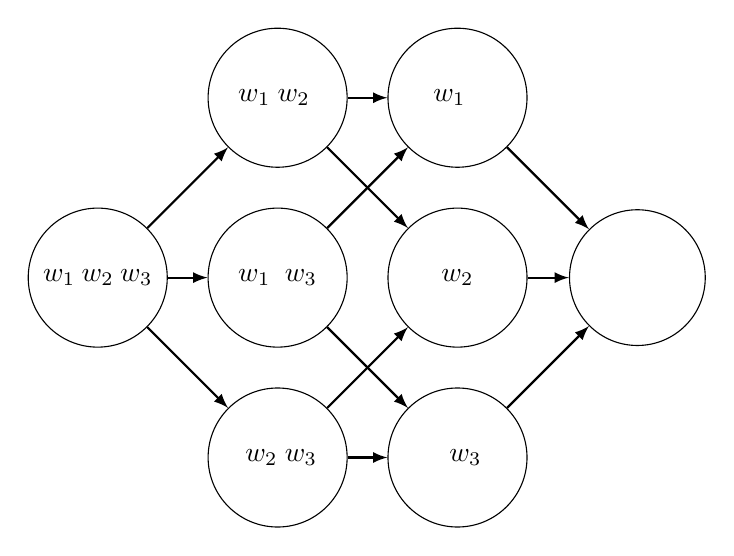
\begin{tikzpicture}[
    node distance = 6.5em,
    seq/.style = {draw, circle, align=center, text centered, text width=4.2em},
  ]
    \node [seq] (000)                {$w_1 \: w_2 \: w_3$};

    \node [seq] (010) [right of=000] {$w_1 \: \Skp \: w_3$};
    \node [seq] (001) [above of=010] {$w_1 \: w_2 \: \Skp$};
    \node [seq] (100) [below of=010] {$\Skp \: w_2 \: w_3$};

    \node [seq] (101) [right of=010] {$\Skp \: w_2 \: \Skp$};
    \node [seq] (011) [above of=101] {$w_1 \: \Skp \: \Skp$};
    \node [seq] (110) [below of=101] {$\Skp \: \Skp \: w_3$};

    \node [seq] (111) [right of=101] {$\Skp \: \Skp \: \Skp$};

    \path[->, >=latex, thick]
      (000) edge (001)
      (000) edge (010)
      (000) edge (100)

      (001) edge (011)
      (001) edge (101)
      (010) edge (011)
      (010) edge (110)
      (100) edge (101)
      (100) edge (110)

      (011) edge (111)
      (101) edge (111)
      (110) edge (111);
  \end{tikzpicture}
\end{figure}

% ------------------------------------------------------------------------------
\begin{landscape}
  \section{Binomial Diamond of order 4}
  \begin{figure}[H]
    \centering
    \scalebox{0.7}{
      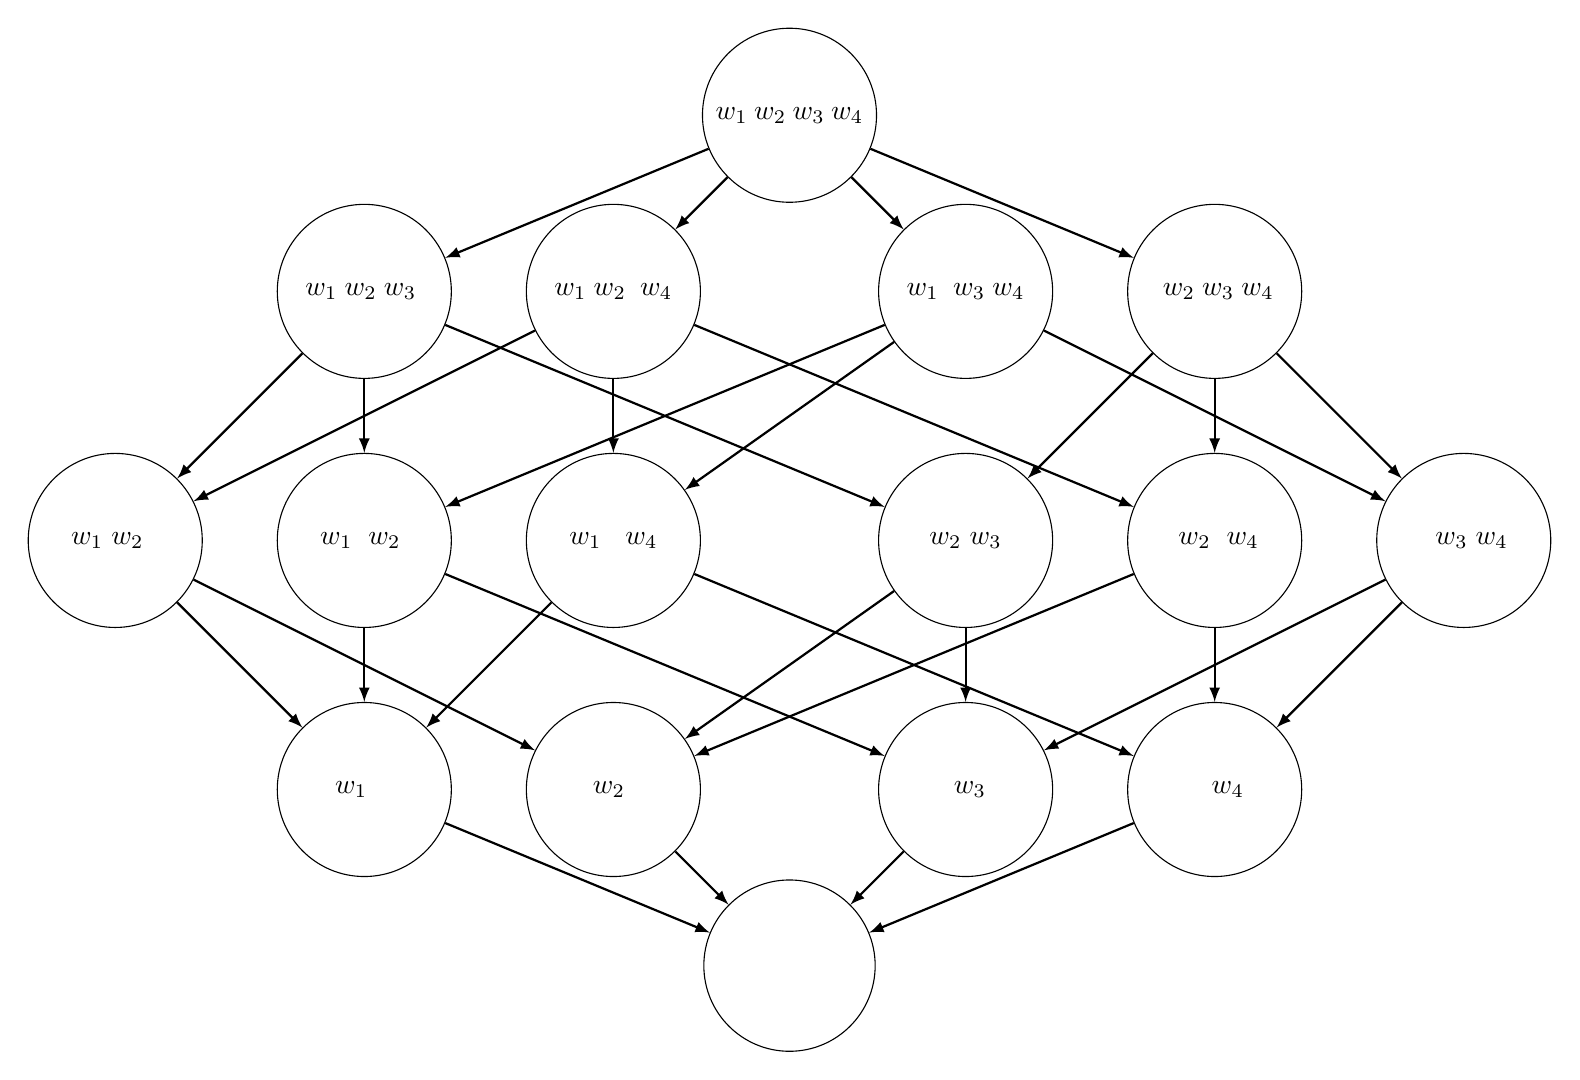
\begin{tikzpicture}[
        node distance = 9em,
        seq/.style = {draw, circle, align=center, text centered, text width=5.5em},
      ]
        \node [seq] (0000) {$w_1 \: w_2 \: w_3 \: w_4$};

        \node [seq] (0010) [below left  of=0000] {$w_1 \: w_2 \: \Skp \: w_4$};
        \node [seq] (0100) [below right of=0000] {$w_1 \: \Skp \: w_3 \: w_4$};
        \node [seq] (0001) [      left  of=0010] {$w_1 \: w_2 \: w_3 \: \Skp$};
        \node [seq] (1000) [      right of=0100] {$\Skp \: w_2 \: w_3 \: w_4$};

        \node [seq] (0101) [below       of=0001] {$w_1 \: \Skp \: w_2 \: \Skp$};
        \node [seq] (0110) [below       of=0010] {$w_1 \: \Skp \: \Skp \: w_4$};
        \node [seq] (1001) [below       of=0100] {$\Skp \: w_2 \: w_3 \: \Skp$};
        \node [seq] (1010) [below       of=1000] {$\Skp \: w_2 \: \Skp \: w_4$};
        \node [seq] (0011) [      left  of=0101] {$w_1 \: w_2 \: \Skp \: \Skp$};
        \node [seq] (1100) [      right of=1010] {$\Skp \: \Skp \: w_3 \: w_4$};

        \node [seq] (0111) [below       of=0101] {$w_1 \: \Skp \: \Skp \: \Skp$};
        \node [seq] (1011) [below       of=0110] {$\Skp \: w_2 \: \Skp \: \Skp$};
        \node [seq] (1101) [below       of=1001] {$\Skp \: \Skp \: w_3 \: \Skp$};
        \node [seq] (1110) [below       of=1010] {$\Skp \: \Skp \: \Skp \: w_4$};

        \node [seq] (1111) [below right of=1011] {$\Skp \: \Skp \: \Skp \: \Skp$};

        \path[->, >=latex, thick]
          (0000) edge (0001)
          (0000) edge (0010)
          (0000) edge (0100)
          (0000) edge (1000)

          (0001) edge (0011)
          (0001) edge (0101)
          (0001) edge (1001)
          (0010) edge (0011)
          (0010) edge (0110)
          (0010) edge (1010)
          (0100) edge (0101)
          (0100) edge (0110)
          (0100) edge (1100)
          (1000) edge (1001)
          (1000) edge (1010)
          (1000) edge (1100)

          (0011) edge (0111)
          (0011) edge (1011)
          (0101) edge (0111)
          (0101) edge (1101)
          (0110) edge (0111)
          (0110) edge (1110)
          (1001) edge (1011)
          (1001) edge (1101)
          (1010) edge (1011)
          (1010) edge (1110)
          (1100) edge (1101)
          (1100) edge (1110)

          (0111) edge (1111)
          (1011) edge (1111)
          (1101) edge (1111)
          (1110) edge (1111);
      \end{tikzpicture}
    }
  \end{figure}
\end{landscape}

% ==============================================================================
\chapter{Timeline}

\begin{itemize}
  \item Write chapters
    \begin{itemize}
      \item Introduction (1-2 days)
      \item Related Work (1 day)
      \item Review of Considered language Models (1 day)
      \item Formulating Language Models as Weighted Sums
      \item Fast Prefix Queries using Top-\emph{k} Joins
      \item Evaluation
      \item Conclusion (1-2 days)
    \end{itemize}
  \item Think of experiments and implement them (3-4 days)
  \item Find new notation for chapter weighted sums (\emph{hard to estimate})
    \begin{itemize}
      \item Needs to be able to nicely represent MKN weighted sum argument.
      \item Should be able to nicely represent GLM weighted sum argument.
      \item It would be nice if the notation makes proving MKN weighted sum.
    \end{itemize}
  \item Finishing (3-4 days)
    \begin{itemize}
      \item Fix latex
      \item Reformulate shitty sentences
      \item Check formatting
    \end{itemize}
  \item Peer review, spelling correction (1-2 weeks)
  \item Make slides, prepare presentation (1 week)
\end{itemize}

\clearpage
\hrule
\subsubsection*{Week 6.7. - 12.7.}
\begin{itemize}
  \item  6.7. Monday:
  \item  7.7. Tuesday:
  \item  8.7. Wednesday:
  \item  9.7. Thursday:
  \item 10.7. Friday:
  \item 11.7. Saturday:
  \item 12.7. Sunday;
\end{itemize}

\hrule
\subsubsection*{Week 13.7. - 19.7.}
\begin{itemize}
  \item 13.6. Monday:
  \item 14.6. Tuesday:
  \item 15.7. Wednesday:
  \item 16.7. Thursday:
  \item 17.7. Friday:
  \item 18.7. Saturday:
  \item 19.7. Sunday;
\end{itemize}

\hrule
\subsubsection*{Week 20.7. - 26.7.}
\begin{itemize}
  \item 20.6. Monday:
  \item 21.6. Tuesday:
  \item 22.7. Wednesday:
  \item 23.7. Thursday:
  \item 24.7. Friday:
  \item 25.7. Saturday:
  \item 26.7. Sunday;
\end{itemize}

\clearpage
\hrule
\subsubsection*{Week 27.7. - 2.8.}
\begin{itemize}
  \item 27.6. Monday: Need to start peer review.
  \item 28.6. Tuesday:
  \item 29.7. Wednesday:
  \item 30.7. Thursday: Need to start working on presentation.
  \item 31.7. Friday:
  \item  1.8. Saturday:
  \item  2.8. Sunday;
\end{itemize}

\hrule
\subsubsection*{Week 3.8. - 9.8.}
\begin{itemize}
  \item  3.8. Monday:
  \item  4.8. Tuesday:
  \item  5.8. Wednesday:
  \item \textbf{6.8. Thursday: Colloquium}
\end{itemize}

\end{appendices}

\listoftodos

\end{document}
